% Variational quantum algorithm: |psi(theta)> = U(theta)|0>^N, cost C(theta) = <psi(theta)|O|psi(theta)>,
% classical optimiser proposes the next theta (notebook 40, Section 1).
\documentclass[tikz,border=4pt]{standalone}
\usepackage{amsmath,amssymb,bm}
\usetikzlibrary{arrows.meta,positioning,calc}
\newcommand{\ket}[1]{\lvert #1\rangle}
\begin{document}
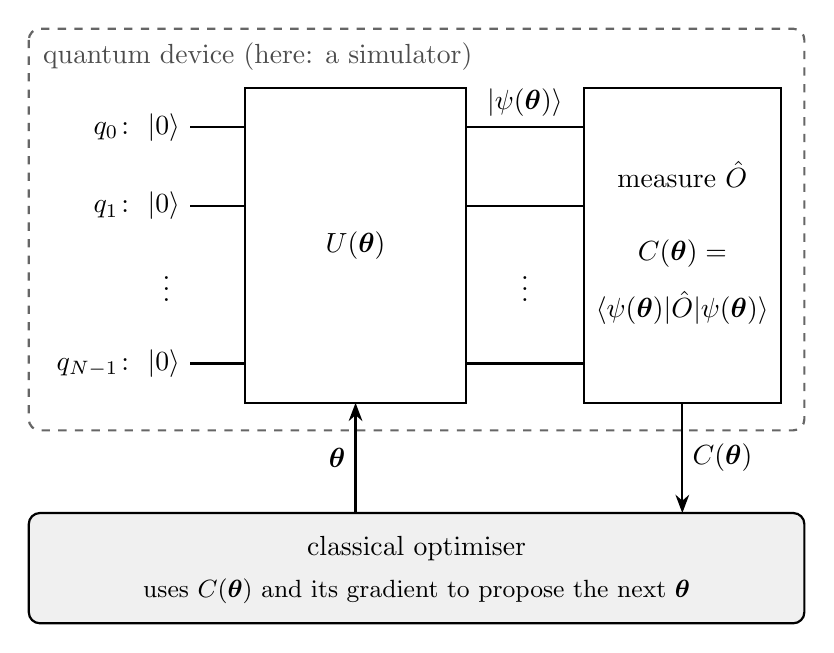
\begin{tikzpicture}[thick, >=Stealth]
  % quantum part (device or simulator)
  \draw[dashed, rounded corners, black!60] (-1.75,1.25) rectangle (8.1,-3.85);
  \node[anchor=north west, black!70] at (-1.7,1.2) {quantum device (here: a simulator)};
  % wires
  \foreach \y/\lab in {0/{q_0}, -1/{q_1}, -3/{q_{N-1}}} {
    \node[anchor=east] at (0.3,\y) {$\lab\colon\ \ket{0}$};
    \draw (0.3,\y) -- (5.3,\y);
  }
  \node at (0.0,-1.95) {$\vdots$};
  \node at (4.55,-1.95) {$\vdots$};
  % the parametrized circuit
  \draw[fill=white] (1.0,0.5) rectangle (3.8,-3.5);
  \node at (2.4,-1.5) {$U(\boldsymbol\theta)$};
  \node[above] at (4.55,0.0) {$\ket{\psi(\boldsymbol\theta)}$};
  % measurement block
  \draw[fill=white] (5.3,0.5) rectangle (7.8,-3.5);
  \node at (6.55,-0.6) {measure $\hat O$};
  \node at (6.55,-1.6) {$C(\boldsymbol\theta)=$};
  \node at (6.55,-2.3) {$\langle\psi(\boldsymbol\theta)\vert\hat O\vert\psi(\boldsymbol\theta)\rangle$};
  % classical optimiser
  \draw[fill=black!6, rounded corners] (-1.75,-4.9) rectangle (8.1,-6.3);
  \node at (3.175,-5.35) {classical optimiser};
  \node at (3.175,-5.9) {\small uses $C(\boldsymbol\theta)$ and its gradient to propose the next $\boldsymbol\theta$};
  % arrows
  \draw[->] (6.55,-3.5) -- node[right]{$C(\boldsymbol\theta)$} (6.55,-4.9);
  \draw[->] (2.4,-4.9) -- node[left]{$\boldsymbol\theta$} (2.4,-3.5);
\end{tikzpicture}
\end{document}
